\section{Auswertung}
\label{sec:Auswertung}
Ein typisches Signalbild der Messung ist in \ref{fig:Signal} dargestellt. Die beiden
Resonanzstellen sind rechts von dem Nullpeak zu finden. Bevor den Resonanzstellen einem
der beiden Rubidium Isotope zugeordnet werden kann, wird der erste Peak rechts von dem Nullpeak
dem \textit{Isotop 1} und der zweite dem  \textit{Isotop 2} zugeordnet.
\begin{figure}
  \centering
  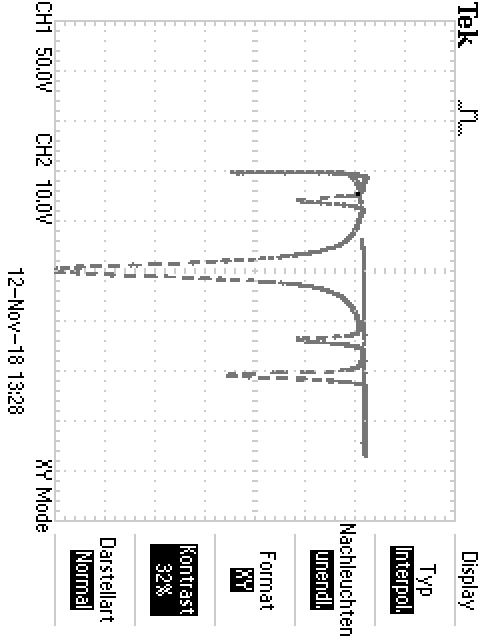
\includegraphics[angle=90]{pics/TEK0000.JPG}
  \caption{Typisches Signalbild auf dem Oszilloskop. Es sind der Nullpeak (mittig) und
           die Resonanzstellen der beiden Isotope zu sehen (rechts).}
  \label{fig:Signal}
\end{figure}
Die Breite des Nullpeaks ist Abhängig von der vertikalen Komponente des Erdmagnetfeldes.
Um den Einfluss der vertikalen Komponente des Erdmagnetfeldes so gering wie möglich zu halten
und damit den Peak zu verschmälern wird der Versuchsaufbau in Nord-Süd-Richtung gedreht und ein
Feld in vertikale Richtung angelegt.
An die vertikal ausgerichtete Helmhotzspule wird ein Strom $I= 0,231$ A angelegt. Damit
ergibt sich mit der magnetischen Feldkonstante $\mu_{0}$, der Windungszahl $N$ der Spule,
dem Radius $R$, dem Strom $I$ und der Helmhotzgleichung
\begin{equation}
  B=\mu_{0}\frac{8 N }{\sqrt{125} R}I
  \label{eq:Helmholz}
\end{equation} eine Feldstärke von $B_{\text{vertikal}}=35,40\,\mu$T.

\subsection{Bestimmung der Landéschen $\text{g}_{\text{F}}$ Faktoren}
Die Einstellungen der Potentiometer sind in Tabelle \ref{tab:Potentiometer} aufgeführt.
\begin{table}[H]
    \centering
    \caption{Auflistung der Potentiometer Werte. Umdrehung 1 bezeichnet dabei die eingestellte Umdrehungszahl der Sweep-Spule für die
    erste Resonanzstelle, Umdrehung 2 die der zweiten und H1 und H2 die Werte des Horizontalfeldes.}
    \label{tab:Potentiometer}
    \begin{tabular}{c|c|c|c|c}
        \toprule
        $f$ in kHz & Umdrehung 1 & Umdrehung 2 & H1 & H2  \\
        \midrule
        100& 5,80 &6,85& 0 & 0 \\
        200& 2,38 &4,78& 0,6& 0,6\\
        300& 1,38 &5,40& 11 &11\\
        400& 3,50 &8,06& 12 &12\\
        500& 2,95 &8,85& 20 &20\\
        600& 0,76 &7,86& 30 &30\\
        700& 0,51 &8,75& 36 &36\\
        800& 1,33 &2,80& 40 &58\\
        900& 1,30  &4,9 &42 &62\\
        1000& 3,80 &5,89& 49& 68\\
        \bottomrule
    \end{tabular}
\end{table}
Die Potentiometerumdrehungen werden mit dem Faktor 0,1A für die Sweep Spulen und
0,03A für die Horizontalspulen in die Stromstärke umgerechnet. Die so berechneten Werte sind in
\ref{tab:Umrechnung} aufgeführt.
\begin{table}[H]
    \centering
    \caption{Auflistung der Stromstärken. $I_{S1}$ bezeichnet dabei die Stromstärke der
    ersten Resonanzstelle, $I_{S2}$ die der zweiten und $I_{H1}$ und $I_{H2}$ die Werte für das Horizontalfeld.}
    \label{tab:Umrechnung}
    \begin{tabular}{c|c|c|c|c}
        \toprule
        $f$ in kHz & $I_1$in A & $I_2$ in A & $I_{H1}$ in A  & $I_{H2}$ in A   \\
        \midrule
        100& 0,580 &0,685& 0 & 0 \\
        200& 0,238 &0,478& 0,018& 0,018\\
        300& 0,138 &0,540& 0,33 &0,33\\
        400& 0,350 &0,806& 0,36 &0,36\\
        500& 0,295 &0,885& 0,6 &0,6\\
        600& 0,076 &0,786& 0,9 &0,9\\
        700& 0,051 &0,875& 1,08 &1,08\\
        800& 0,130 &0,280& 1,2 &1,74\\
        900& 0,130  &0,49 &1,26 &1,86\\
        1000& 0,380 &0,589& 1,47& 2,04\\
        \bottomrule
    \end{tabular}
\end{table}
Daraus lässt sich mit Formel \ref{eq:Helmholz} die Magnetfeldstärke bestimmen.
Dabei sind die Radien der Spulen $R_{S}=11$ und $R_H=154$Die
so gewonnenen Werte sind in Tabelle \ref{tab:Magnetwerte} aufgeführt.
\begin{table}[H]
    \centering
    \caption{Auflistung der Magnetfeldstärken. $B_1$ bezeichnet dabei die Stromstärke der
    ersten Resonanzstelle, $B_2$ die der zweiten und $B_{H1}$ und $B_{H2}$ die Werte für das Horizontalfeld.}
    \label{tab:Magnetwerte}
    \begin{tabular}{c|c|c|c|c}
        \toprule
        $f$ in kHz & $B_1$ in T & $B_2$ in T& $B_{H1}$ in T& $B_{H2}$ in T \\
        \midrule
        100& 35,00 & 41,34& 0 & 0 \\
        200& 14,36 &28,85& 1,09& 1,09\\
        300& 8,33 &32,59& 19,91&19,91\\
        400& 21,12 &48,64& 21,73&21,73\\
        500& 17,80 &53,41&  36,21& 36,21\\
        600& 4,59 &47,43& 54,31 &54,31\\
        700& 3,08 &52,80& 65,18 &65,18 \\
        800& 8,03 &16,90& 72,42 & 105,00\\
        900& 7,84  &29,57 & 76,04&112,25\\
        1000& 22,94 &35,54& 88,71& 123,11\\
        \bottomrule
    \end{tabular}
\end{table}
Die Magnetfeldstärken $B_1$ und $B_{H1}$ sowie $B_2$ und $B_{H2}$ werden zu den Gesamtfeldstärken
$B_1$ und $B_2$ addiert.
Zwischen der Magnetfeldstärke $B$ und der Frequenz $f$ an den Resonanzstellen besteht der Zusammenhang
\begin{equation}
  B=\frac{\text{h}f}{\mu_{\text{B}} \text{g}_{\text{F}}} .
\end{equation}
Dieser Zusammenhang ist in \ref{fig:BFelder} aufgeführt. Es wurde eine Gerade der
Form $y=m\cdot x+b$ an die Messwerte der beiden Isotope gefittet. Die Fitparameter sind dabei
\begin{align*}
  m_1&=(0,09 \pm 0,01)\,\frac{\mu\text{T}}{\text{kHz}} \\
  b_1&=(7 \pm 6)\,\mu\text{T}\\
  m_2&=(0,142 \pm 0,008)\,\frac{\mu\text{T}}{\text{kHz}} \\
  b_2&=(15 \pm 5)\,\mu\text{T}
\end{align*}
\begin{figure}
  \centering
  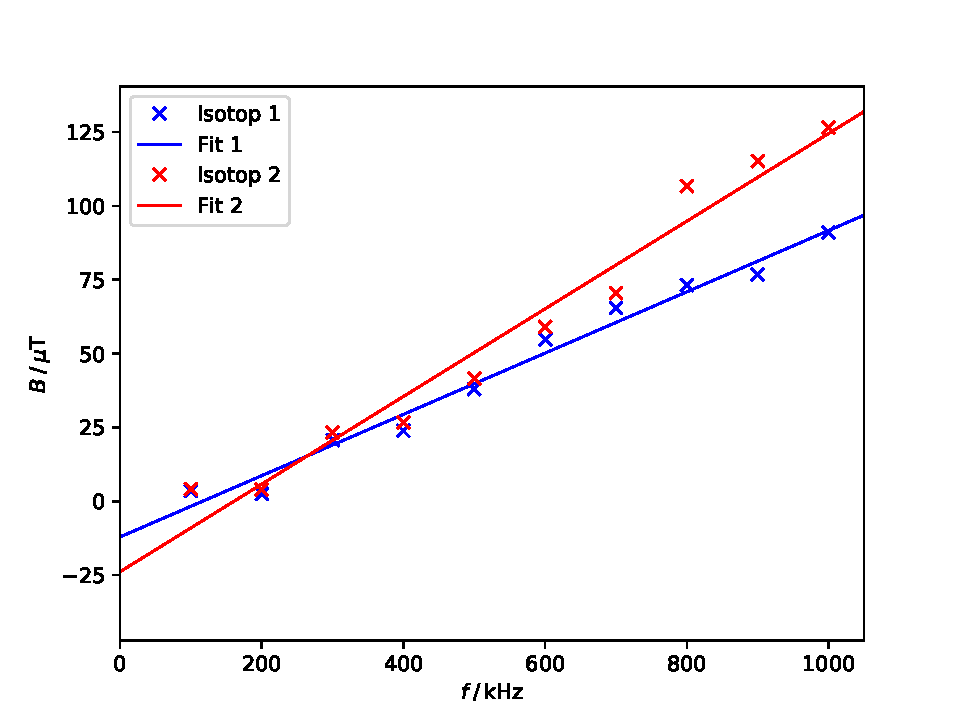
\includegraphics{plots/BFelder.pdf}
  \caption{Die Stärke des Magnetfeldes gegen die Resonanzfrequenzen für die beiden Isotope
  aufgetragen.}
  \label{fig:BFelder}
\end{figure}
Daraus lassen sich die Landéschen $\text{g}_{\text{F}}$ Faktoren mit
\begin{equation}
  \text{g}_{\text{F}}=\frac{\text{h}}{\mu_{\text{B}}} \frac{f}{B}
\end{equation}
bestimmen, wobei das Verhältnis von Magnetfeld uns Frequenz durch die
Steigung $m=B/f$ aus dem Fit von \ref{fig:BFelder} ausgedrückt werden kann.\\
Damit lassen sich die Landéschen $\text{g}_{\text{F}}$ Faktoren zu:
\begin{align*}
  \text{g}_{\text{F,1}}&=0,78 \pm 0,09 \\
  \text{g}_{\text{F,2}}&= 0,50 \pm 0,03
\end{align*}
berechnen.\\
Das Verhältnis der beiden Faktoren ist
\begin{equation}
  \frac{\text{g}_{\text{F,1}}}{  \text{g}_{\text{F,2}}}= 1,6 \pm 0,2.
\end{equation}
Um den Kernspin der Rubidium Isoptope zu berechnen werden die Quantenzahlen $L$,
$S$ und $J$ benötigt.
Diese sind
\begin{align*}
  L&=0\\
  S&=\frac{1}{2}\\
  J&=\frac{1}{2}
\end{align*}
Für die Berechnung der Kernspins wird die Formel \ref{eq:gF} nach $I$ umgestellt.
Desweiternen ergibt sich aus den Werten für $L,S$und $J$ $g_J = 2.0023$. Die Formel \ref{eq:gJ} lässt sich nach $I$ umstellen:
\begin{equation}
  \text{I} = \frac{g_J}{2g_F}-\frac{1}{2} .
  \label{eq:kernspin}
\end{equation}.
Daraus ergeben sich die Werte für den Kernspin der Isotope zu:
\begin{align*}
  I_1& = 0,8 \pm 0,2\\
  I_2&= 1,5 \pm 0,1
\end{align*}
Ausgehend davon, dass die Messung für $I_2$ innerhalb des Fehlerintervalls zu
dem Literaturwert von $\symup{^{87}Rb}$ passt, ließe sich vermuten, das es sich um dieses
Isotop handelt.
Die Literaturwerte für $\symup{^{85}Rb}$ ist $I=\frac{5}{2}$ und für $\symup{^{87}Rb}$ $I=\frac{3}{2}$.
Da beide Isotope vorkommen, wird vermutet, dass das Isotop mit dem geringeren Wert, also
$I_1$ $\symup{^{87}Rb}$ ist und das $I_2$ dementsprechend $\symup{^{87}Rb}$.
\subsection{Bestimmung des Isotopenverhältnisses}
Aus dem Verhältnis der Amplituden der Resonanzstellen lässt sich auf das Isotopenverhältnis schließen.
In Abbildung \ref{fig:Ampli} sind die ausgemessenen Resonanzen bei $100\,$kHz dargestellt.
\begin{figure}
  \centering
  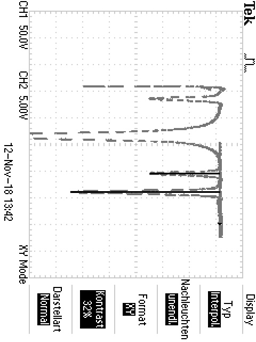
\includegraphics[angle=90]{pics/VerhltnisAmpli.JPG.png}
  \caption{Signalbild bei 100 kHz mit eingezeichneten Amplituden der Resonanzen.}
  \label{fig:Ampli}
\end{figure}
Die Amplituden wurden mittels Pixelzählung vermessen, dabei wurde ein Ablesefehler von
einem Prozent angenommen. Es ergeben sich folgenede Längen:
\begin{align*}
  A_{I1} &= 70,51 \pm 0,7 \text{px}\\
  A_{I2} &= 149,33 \pm 1,5\text{px} .
\end{align*}
Das Verhältnis entspricht
\begin{equation}
  \frac{A_{I1}}{A_{I2}}= 0,47 \pm 0,01.
\end{equation}
\subsection{Abschätzung des quadratischen Zeemaneffekts}
Mittels der Gleichung \ref{eq:quadZ} lässt sich eine Abschätzung für den
quadratischen Zeemaneffekt geben.
Dazu werden die größten gemessenen Magnetfeldwerte für die Abschätzung verwendet.
Das sind für $\symup{^{87}Rb}$ $B_1=91,0\,\mu$T und für $\symup{^{85}Rb}$ $B_2=126,6\,\mu$T.
Die Abstände der Niveaus der Hyperfeinstrukturaufspaltung lauten
$\Delta E_{hy} = 4.53\cdot 10^{-24}\si{\joule}$ für
$\symup{^{85}Rb}$ und $\Delta E_{hy} = 2.01\cdot 10^{-24}\si{\joule}$ für $\symup{^{87}Rb}$ \cite{Anleitung}.
Außerdem werden die magnetischen Quantenzahlen $\symup{M_F} = 3$ für
$\symup{^{85}Rb}$ und $\symup{M_F} = 2$ für $\symup{^{85}Rb}$.
Diese Werte ergeben sich aus dem Kernspin und dem Spin der Elektronenhüllen.\\
Damit ergibt sich für $\symup{^{85}Rb}$
\begin{equation}
  U_{\text{HF,85}}=(7,4\pm0,4)10^{-28},
\end{equation}
und für
$\symup{^{87}Rb}$
\begin{equation}
  U_{\text{HF,87}}=(8,1 \pm 0,9)10^{-28} .
\end{equation}
\subsection{Untersuchung der transienten Effekte}
Ein typisches Siganlbild dieser Messung ist in Abbildung \ref{fig:trans} zu finden.
\begin{figure}
  \centering
  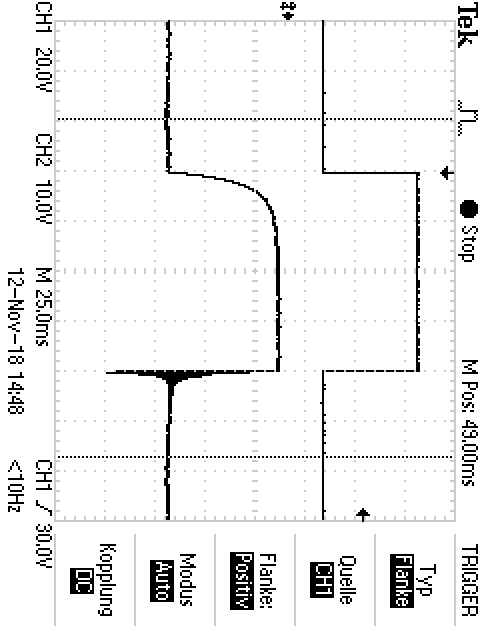
\includegraphics[angle=90]{pics/TEK0033.JPG}
  \caption{Typisches Signalbild der Messung zur Untersuchung der transienten Effekte.}
  \label{fig:trans}
\end{figure}
In den Abbildungen \ref{fig:transfit1} und \ref{fig:transfit2} sind die Periode
gegen die RF-Amplitude aufgetragen.
Eine Hyperbel-Funktion der Form
\begin{equation}
  f(x)=a+\frac{b}{x-c}
\end{equation}
wird zur Ausgleichsrechnung benutzt.
\begin{figure}
    \centering
    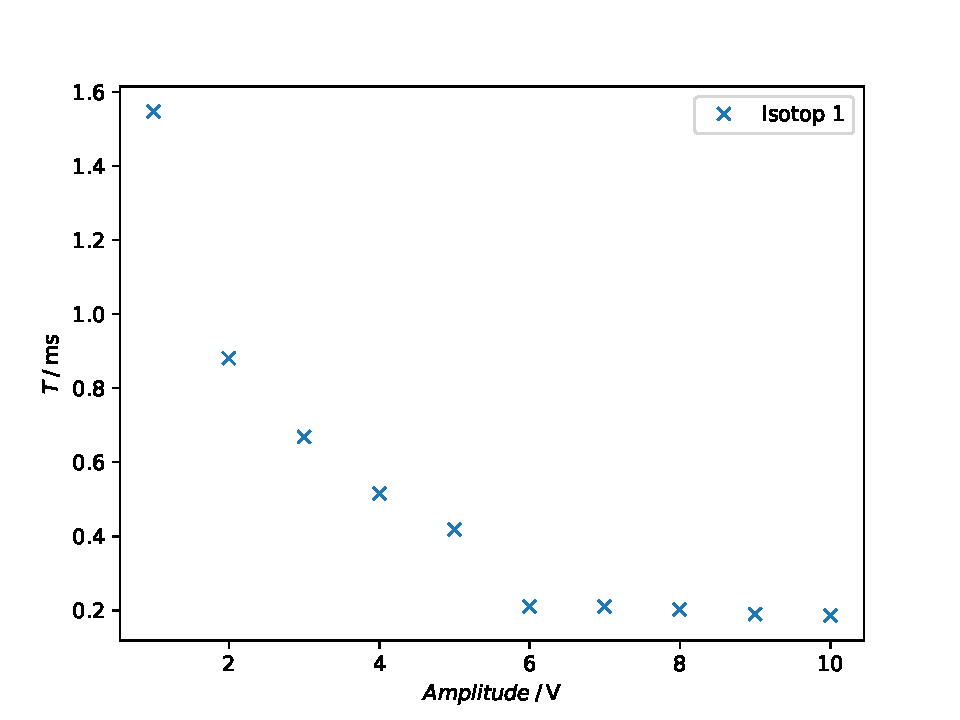
\includegraphics[width=0.8\linewidth]{plots/Trans1.pdf}
    \caption{Die RF-Amplitude gegen die Periode sind samt Ausgleichskurve dargestellt für das
    Isotop $\symup{^{87}Rb}$.}
    \label{fig:transfit1}
\end{figure}
\begin{figure}
  \centering
  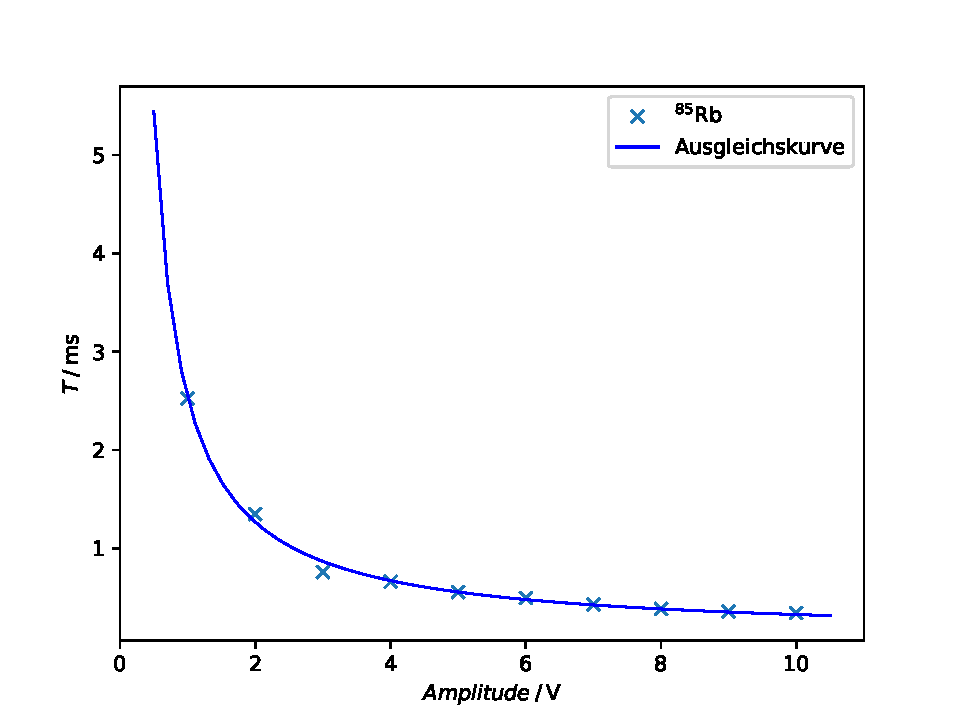
\includegraphics[width=0.8\linewidth]{plots/Trans2.pdf}
  \caption{Die RF-Amplitude gegen die Periode sind samt Ausgleichskurve dargestellt für das
  Isotop $\symup{^{85}Rb}$.}
  \label{fig:transfit2}
\end{figure}
Die Parameter der Ausgleichsrechnung von \ref{fig:transfit1} sind:
\begin{align*}
  a&=(-0,10 \pm 0,06)\,\symup{ms}\\
  b&=(2,7 \pm 0,5)\,\frac{\symup{V}}{\symup{ms}}\\
  c&=(0,6 \pm 0,3)\,\symup{V}
\end{align*}
Die Parameter der Ausgleichsrechnung von \ref{fig:transfit2} sind:
\begin{align*}
  a&=(0,10 \pm 0,05)\,\symup{ms}\\
  b&=(2,2 \pm 0,3)\,\frac{\symup{V}}{\symup{ms}}\\
  c&=(-0,08 \pm 0,10)\,\symup{V}
\end{align*}
Damit lässt sich das Verhältnis
\begin{equation}
  \frac{b(\symup{^{87}Rb})}{b(\symup{^{85}Rb})} = (1,2\pm0,3)
\end{equation}
bestimmen.
% \begin{table}
%    % Notation :  {% nicht entfernen ist sehr wichtig sonst Fehler !!
% \parbox{0.48\textwidth}{% %Ermöglicht zwei Tabellen neben einander
%   \centering
%   \sisetup{round-mode = places , round-precision = 0,scientific-notation=fixed, fixed-exponent = 0}
%          %rundet Werte aus Stelle, Stelle = ,  macht einen bestimmten festen exponenten
%   \resizebox{\textwidth}{!}{%  % skaliert zu große Tabellen
%   \begin{tabular}{S@{${}\pm{}$} S} % fügt plus minus Fehler Schreibweise hinzu
%     \toprule
%      $\text{e}_b / \si{\milli\meter}$ &
%      $\text{d}_b /\si{\milli\meter} $ & $\text{f}_b / \si{\milli\meter} $\\
%     \midrule
%     \bottomrule
%   \end{tabular}
%   % }
%   \caption{Tabellenunterschrift}
%   \label{tab:tab}
% }
% % \end{table}
% % \begin{table}
% \parbox{0.48\textwidth}{%
%   \centering
%   \sisetup{round-mode = places , round-precision = 0,scientific-notation=fixed, fixed-exponent = 0}
%   % \resizebox{\textwidth}{!}{%
%   \begin{tabular}{S@{${}\pm{}$} S}
%     \toprule
%      $\text{e}_b / \si{\milli\meter}$ &
%      $\text{d}_b /\si{\milli\meter} $ & $\text{f}_b / \si{\milli\meter} $\\
%     \midrule
%     \bottomrule
%   \end{tabular}
%   % }
%   \caption{Tabellenunterschrift}
%   \label{tab:tab}
% }
% \end{table}
